Our method allows the specification of a reference family rather than requiring a single reference drift. And it facilitates sharing of information between time intervals. In what follows, we first describe a general optimization setup allowing a reference family. We then establish theoretical guarantees for an iterative approach to solving the optimization. Finally, we provide a practical algorithm that reflects this approach.


\textbf{Optimization with a reference family.} We first generalize the optimization problems from \cref{eq:SBP-main,eq:SBP-drift} to allow a reference family. Let $\modelfamily$ be the chosen reference family of densities over trajectories. Then we replace \cref{eq:SBP-main} with:
\begin{align}
    \label{eq:SB_obj}
    \argmin_{\bridge\in \measurefamily} \min_{\substack{\refden\in\modelfamily:\\ \bridge_{0} = \refden_{0}}}
    \KL(\bridge||\refden),
\end{align}
which reduces to \cref{eq:SBP-main} when $\modelfamily$ has a single element.
Next we restrict the elements of the reference family to be distributions over trajectories implied by the SDE in \cref{eq:mainsde}, with shared volatility $\volatility$. As before, it must be the case that the minimizer of \cref{eq:SB_obj} also solves an SDE of the form in \cref{eq:mainsde}, with the same volatility $\volatility$. So we can write $\refden=\refden_{\refdrift}$ and $\bridge=\bridge_{\modeldrift}$. Then solving \cref{eq:SB_obj} is equivalent to solving for the optimal drift:
%\TB{TB writes: put correct macros in here:}
\begin{align}
    \label{eq:SBP_obj_drift}
    \argmin_{\modeldrift: \bridge_{\modeldrift} \in \measurefamily} \min_{\substack{\refdrift:\refden_{\refdrift}\in\modelfamily,\\\bridge_{\modeldrift,0}=\refden_{\refdrift,0}}} \KL(\bridge_{\modeldrift}||\refden_{\refdrift} )
\end{align}


\textbf{An iterative approach.} To solve the optimization problem in \cref{eq:SBP_obj_drift}, we propose an iterative approach. Namely, we propose to iterate between the following two steps after initializing with some $\refdrift^{(0)}$ and $\iteralgo=1$. %\TB{TB writes: check usage of macros here}
\begin{align}
    \drift^{(\iteralgo)} &= \argmin_{ \drift: \bridge_{\drift} \in \measurefamily} \, \KL(\bridge_{\drift} \| \refden_{\refdrift^{(\iteralgo-1)}})\label{eq:first-proj}\\
    \refdrift^{(\iteralgo)} &= \argmin_{\refdrift: \refden_{\refdrift}\in\modelfamily} \, \KL(\bridge_{\drift^{(\iteralgo)}} \| \refden_{\refdrift})\label{eq:second-proj}
\end{align}

By construction, this iterative scheme will monotonically decrease the objective in \cref{eq:SBP_obj_drift} at each step. Our next result shows that, under additional assumptions, the scheme converges to the optimum.
%%%
\begin{restatable}{myProposition}{iterkl}
\label{prop:iter-kl}
Suppose $\modelfamily$ is a convex set of densities over trajectories implied by the SDE in \cref{eq:mainsde}; suppose all densities have shared volatility $\volatility$ and the same marginal distribution at time $0$.
Suppose that all SDEs satisfy~\cref{assumption-lipschitz,assumption-bddsecondmoments}.
Suppose $\exists C < \infty$ such that, for every drift $\drift$ with $\bridge_{\modeldrift} \in \measurefamily$ or $\refden_{\modeldrift}\in\modelfamily$,
\begin{align*}
&\sup_{(x,t) \in \mathbb{R}^n \times [0,\timestep{\totsteps}]} \| \drift(x, t)\|_{\infty} \leq C 
\end{align*}
Take any initialization $\refdrift^{(0)}$. If $\drift^{(\iteralgo)}$ and $\refdrift^{(\iteralgo)}$ are computed by recursively applying \cref{eq:first-proj,eq:second-proj}, we have
\[
    \lim_{\iteralgo \to \infty} \KL(\bridge_{\drift^{(\iteralgo)}} \| \refden_{\refdrift^{(\iteralgo)}}) = \inf_{\substack{\bridge_{\drift} \in \measurefamily \\ \refden_{\refdrift} \in \modelfamily}} \KL(\bridge_{\drift} \| \refden_{\refdrift})
\]
\end{restatable}
%%%
We prove this result in \cref{app:iter_proj_theory} by adapting standard arguments from the theory of iterative projections \citep{csiszar1975divergence, csiszar2004information, benamou2015iterative}. Along the way, we prove and use that $\measurefamily$ is convex (\cref{lemma:convexD}). We do not necessarily expect the reference family $\modelfamily$ to be convex though. In practice, then, our result guarantees convergence to a local, rather than global, minimum of the KL. We also note that convergence of the KL need not imply convergence of the arguments of the KL; see \cref{sec:identifiability} for further discussion of potential identifiability issues.


\textbf{A practical algorithm.}
We cannot solve \cref{eq:first-proj,eq:second-proj} exactly. We next detail how we derive approximate solutions, $\estimatedriftstep{{(\iteralgo)}}$ and $\estimaterefdriftstep{{(\iteralgo)}}$. We summarize our full method in Algorithm~\ref{algo:sb-irr-algo}.

\SetKwComment{Comment}{/* }{ */}
\begin{algorithm}[!t]
    \caption{Our method iterates between (1) estimating the forward and backward bridge drifts given the current best reference guess and (2) using simulated trajectories from the current bridge drift estimates to find a new best reference guess.}
    \label{algo:sb-irr-algo}
    \KwIn{ 
    $\{\obsatall{\timestep{\timeidx}}\}_{\timeidx=1}^{\totsteps}$,
    iteration count $K$, $\Delta \timet$}
    
    $\estimaterefdriftstep{(0)} \gets 0$, $k\gets 0$\ \\
    \While{ $k<K$}{
        $\iteralgo = \iteralgo+1$ \\
        \For{$i=1,\dots,\totsteps-1$}{
            $\estimatedriftstep{\timeidx(\iteralgo)},\estimatebackwarddriftstep{\timeidx(\iteralgo)}=\textrm{\texttt{Forward-Backward-SB}}(\obsatall{\timestep{\timeidx}}, \obsatall{\timestep{\timeidx+1}}||\estimaterefdriftstep{(\iteralgo-1)})$\ 
        }
        $\textrm{SampleTrajectories}=\{\}$\ 
        
        \For{$\timeidx=1,\dots,\totsteps-1$}{
        \For{$\sampleidx_{\timeidx}=1,\dots,\tottrajec_{\timestep{\timeidx}}$}{
            
            $\simulatedresponseat{0\le \timet\le \timestep{\timeidx}}^{(i,\sampleidx_{\timeidx})}\!= \textrm{\texttt{backwardSDE}}(\estimatebackwarddriftstep{(\iteralgo)}, \obsat{\timestep{\timeidx}}^{\sampleidx_{\timeidx}},\Delta \timet)$ 
            
            $\simulatedresponseat{\timestep{\timeidx}< \timet\le \timestep{\totsteps}}^{ (i,\sampleidx_{\timeidx}) }=\textrm{\texttt{forwardSDE}}(\estimatedriftstep{(\iteralgo)}, \obsat{\timestep{\timeidx}}^{\sampleidx_{\timeidx}},\Delta \timet)$
            
            SampleTrajectories.append($\simulatedresponseat{0 \le \timet\le \timestep{\totsteps}}^{(i,\sampleidx_{\timeidx}) }$)
            
        }
        }
        $\estimaterefdriftstep{{(\iteralgo)}} \gets$ \textrm{\texttt{MLEfit}}(SampleTrajectories)
    }
    \KwOut{$\estimatedriftstep{(K)}, \estimatebackwarddriftstep{(K)}$ to generate trajectories}
\end{algorithm}

\textbf{Algorithm step 1.} First, consider \cref{eq:first-proj}, where we optimize the bridge model given the current reference. This step is a multi-marginal SB problem, with reference dynamic $\refden_{\estimaterefdriftstep{{(\iteralgo)}}}$. As discussed above, the problem reduces to standard SB problems pairwise between time points. There are many implementations that approximately solve the SB problem: e.g., a regression method \citep{Vargas2021}, score matching \citep{wang2021deep}, or a proximal method \citep{Caluya2022}. We denote an implementation's output between time points $\timestep{\timeidx}$ and $\timestep{\timeidx+1}$ as $\estimatedriftstep{\timeidx(\iteralgo)},\estimatebackwarddriftstep{\timeidx(\iteralgo)}=\textrm{\texttt{Forward-Backward-SB}}(\obsatall{\timestep{\timeidx}}, \obsatall{\timestep{\timeidx+1}}||\refdrift^{(\iteralgo-1)})$. 
In our code implementation, we follow the regression-based method of \citet{Vargas2021}; see \cref{sec:first_projection_implementation}.
However, our framework is in principle compatible with any solver that (i) supports a general reference measure beyond Brownian motion and (ii) outputs forward and backward drifts for the particle evolution. For a more comprehensive discussion of alternative methods for this step, we refer the reader to \cref{app:sb-methods-discussion}.

\textbf{Algorithm step 2.} The second problem, \cref{eq:second-proj}, does not arise in standard SBs. Our proposed methodology for an approximate solution has two parts, which we detail below: (i) we sample trajectories given the forward and backward bridge drift estimates from the first step, and (ii) we solve a maximum likelihood problem given these sample trajectories.

\begin{figure*}[!ht]
    \centering
    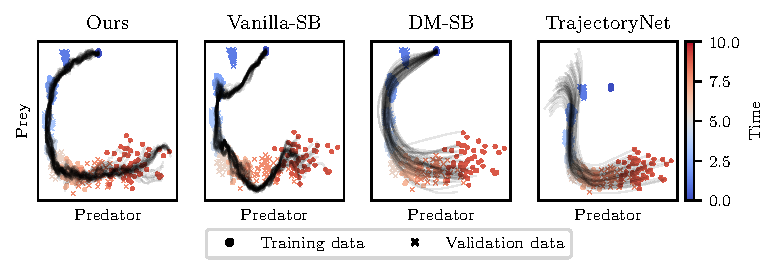
\includegraphics[width =.95\textwidth]{Figs/LV50_trajectories.pdf}
    \caption{Comparison on the Lotka-Volterra synthetic data (\cref{sec:LVmain}) with 5 training times, 4 validation times, and 50 observations per time. Each plot shows 50 simulated trajectories, originating from particles at one time end point (three left plots: first time; right plot: final time); see ``Measuring Accuracy'' in \cref{sec:experiments-main}.  
    }
    \label{fig:LV-main}
\end{figure*}

\textbf{Algorithm step 2.i.} From step 1, we have forward and backward bridge drift estimates $\estimatedriftstep{(\iteralgo)},\estimatebackwarddriftstep{(\iteralgo)}$. Recall ``Generating sample trajectories'' within \cref{sec:setup}; for each observation $\obsat{\timestep{\timeidx}}^{\sampleidx_{\timeidx}}$, we can simulate a trajectory in $\timet \in [0,\timestep{\totsteps}]$ via $\simulatedresponseat{0\le \timet\le \timestep{\timeidx}}^{(i,\sampleidx_{\timeidx})}= \textrm{\texttt{backwardSDE}}(\estimatebackwarddriftstep{(\iteralgo)}, \obsat{\timestep{\timeidx}}^{\sampleidx_{\timeidx}},\Delta \timet)$ and $\simulatedresponseat{\timestep{\timeidx}< \timet\le \timestep{\totsteps}}^{ (i,\sampleidx_{\timeidx}) }=\textrm{\texttt{forwardSDE}}(\estimatedriftstep{(\iteralgo)}, \obsat{\timestep{\timeidx}}^{\sampleidx_{\timeidx}},\Delta \timet)$. Then we have $\totalnumparticles$ simulated trajectories.

\textbf{Algorithm step 2.ii.}
By expanding $\KL$ and dropping terms where $\refden_{\refdrift}$ does not appear, we can rewrite \cref{eq:second-proj} as follows; see \cref{app:inverseproj} for full details and derivation of this step of the algorithm. 
\begin{align}
    \refdrift^{(\iteralgo)} &= \argmin_{\refdrift: \refden_{\refdrift}\in\modelfamily} \, \KL(\bridge_{\drift^{(\iteralgo)}} \| \refden_{\refdrift}) \\
    &= \argmax_{\refdrift: \refden_{\refdrift}\in\modelfamily} \mathbb{E}_{\bridge_{\drift^{(\iteralgo)}}} \log \refden_{\refdrift}
    \label{eq:max_likelihood}
\end{align}
We can approximate the exact objective in \cref{eq:max_likelihood}
by replacing the expectation $\mathbb{E}_{\bridge_{\drift^{(\iteralgo)}}}$ with an empirical average over the trajectories $\{\simulatedresponseat{0\le \timet\le \timestep{\totsteps}}^{(\timeidx,\sampleidx_{\timeidx})}\}_{\timeidx,\sampleidx_{\timeidx}}$, which are simulated from $\bridge_{\drift^{(\iteralgo)}}$. The resulting optimization problem over this approximate objective can be seen as maximizing the (log) likelihood of the simulated trajectories $\{\simulatedresponseat{0\le \timet\le \timestep{\totsteps}}^{(\timeidx,\sampleidx_{\timeidx})}\}_{\timeidx,\sampleidx_{\timeidx}}$ over the choice of $\refdrift$ in $\refden_{\refdrift}$.
Since the simulated trajectories are obtained by a standard Euler-Maruyama approach with sampling rate $\Delta t$, they can be represented by a Gaussian autoregressive process.
We show in \cref{app:inverseproj} that the optimization problem therefore reduces to a least squares scheme, where the square errors arise from the Gaussian log likelihoods. Given the connection to maximum likelihood estimation (MLE), we let \texttt{MLEfit} denote the function that takes in sample trajectories and outputs our resulting estimate $\estimaterefdriftstep{(\iteralgo)}$ of the reference drift $\refdrift^{(\iteralgo)}$.